\documentclass[mathserif]{beamer}
%\usefonttheme{serif}
\usepackage[utf8]{inputenc}
\usepackage[T1]{fontenc}
\usepackage{lmodern}
\usepackage{etoolbox}
\usepackage{graphicx}
\usepackage{xcolor}
\usepackage{transparent}
\usepackage{hyperref}
\usepackage{amsmath}
\usepackage{tcolorbox}
\usepackage{parskip}
\usepackage[framemethod=tikz]{mdframed}
\usepackage{mathrsfs}
\usepackage{physics}
\usepackage{tikz, tikz-cd}
\usepackage[citestyle=nature]{biblatex}
\usepackage{tensor}
\usepackage[absolute,overlay]{textpos}
\newcommand{\e}{\mathrm{e}}

\renewcommand\thefootnote{\textcolor{red!50!white}{\arabic{footnote}}}

\newcommand\FrameText[1]{%https://tex.stackexchange.com/a/32990/191229
	\begin{textblock*}{\paperwidth}(0pt,\textheight)
		\vspace{-2em}
		\raggedleft #1\hspace{2em}
\end{textblock*}}


\setbeamercolor{background canvas}{bg=black}
\usebackgroundtemplate{\tikz[overlay,remember picture] \node[opacity=1, at=(current page.center)] {
\includegraphics[height=\paperheight]{img/bakgrunn_plain.png}};
\FrameText{\href{https://www.twitter.com/Karlockert}{{\transparent{0.4}{@karlockert}}}}
}


\setbeamertemplate{footline}[frame number]{}
% Fjerner navigasjonsbaren nederst
\setbeamertemplate{navigation symbols}{}
% Fjerner navigasjonssymbolene

\begin{document}
	\color{white}
%	%\usebackgroundtemplate{%             declare it
%	\tikz[overlay,remember picture] \node[opacity=1, at=(current page.center)] {
%		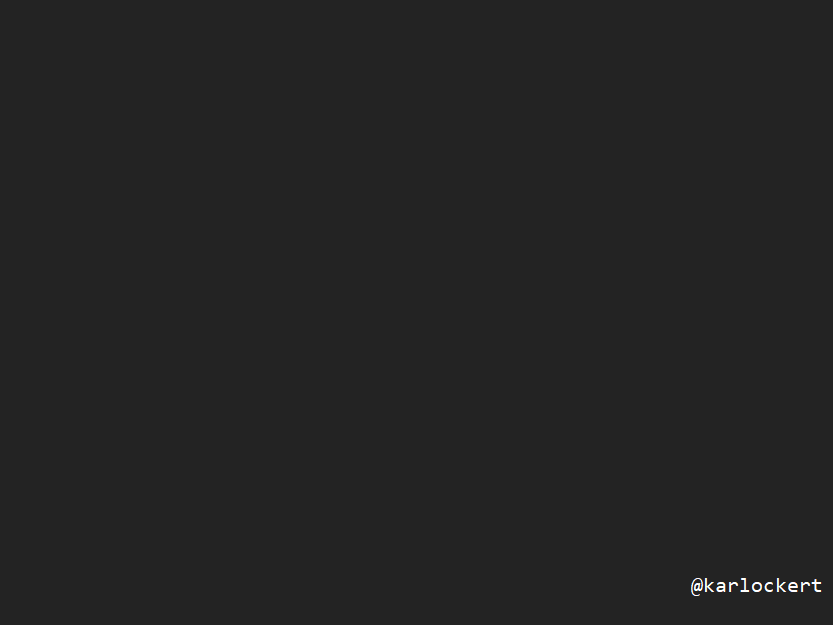
\includegraphics[height=\paperheight]{img/bakgrunn.png}};}

\begin{frame}[noframenumbering, plain]
	\begin{block}{\color{white}\textbf{\Large{
				%
					Title goes here
			%	
			}}}
		\vspace{-10pt}\rule{\textwidth}{0.5pt}
		\color{white}
		
		Some information about a cool theorem or anything i find interesting, related equations (here: Dirac-equation)
	
	\end{block}
	{\large
		
		\begin{equation*} 
			(i\gamma_{\mu}\partial^{\mu} - m)\psi = 0
		\end{equation*}
	}

	\begin{block}{}
	\color{white}
	
		Some more information here
		
	\end{block}
	

\end{frame}
	% Laget av: person

%\usebackgroundtemplate{%             declare it
%	\tikz[overlay,remember picture] \node[opacity=1, at=(current page.center)] {
%		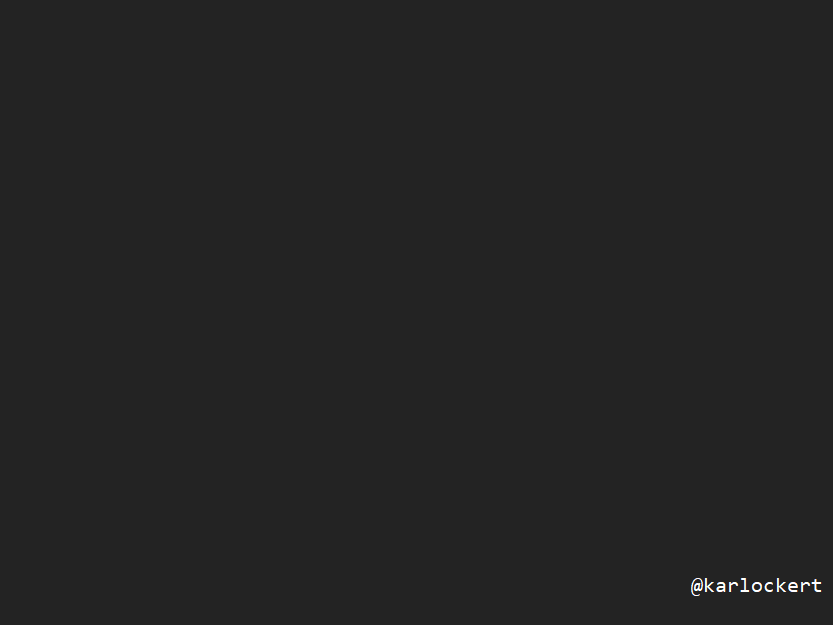
\includegraphics[height=\paperheight]{img/bakgrunn.png}};}
% Sett inn dit custom bilde her. template_background.png har riktig dimensjon, så om man vil redigere er det letteste å laste ned denne filen og redigere.

\begin{frame}[noframenumbering, plain]
	%	\frametitle{Hvis du ønsker}
	
	\begin{block}{\color{white}\textbf{\Large{Ehrenfests teorem }}}
		\vspace{-10pt}\rule{\textwidth}{0.5pt}
		\color{white}
		Hvorfor kollapser ikke bølgefunksjonen til hverdagslige ting (som f.eks. en stol)? Korrespondanseprinsippet forteller oss at i grensen av store antall partikler og høye energier, må kvantemekanikk være ekvivalent med klassisk fysikk. 
		Paul Ehrenfest fant en måte å relatere tidsutviklingen i forventningsverdien av kvantemekaniske operatorer til forventningsverdien av kraften som virker på systemet. Fra Newtons andre lov er dette forventet, men Ehrenfests teorem gir en matematisk trygghet. En generalisering av teoremet kan skrives på formen
	\end{block}
	{\large
		
		\begin{equation*} 
			\dv{t}\ev{O} = 	-i\hbar\ev{\comm{O}{\mathcal{H}}} + \ev{\pdv{O}{t}}	
		\end{equation*}
	}
	
	\begin{block}{}
		\color{white}
	hvor $O$ er en operator som korresponderer til en observerbar størrelse og $\mathcal{H}$ er Hamiltonian til systemet.
	\end{block}
\end{frame}

	
	
\end{document}

